\chapter{FEM Mesh Refinement for 3D EIT}
\label{chap:chapter-4}

\section{Motivation}
This thesis proposes the use of novel 3D electrode configurations 
and internal electrodes to improve sensitivity to 
cardiosynchronous activity. Unlike surface electrode configurations, these 
modles have a very high 
sensitivity in the center of a model where mesh refinement can be challenging. 
In this chapter we explore the need for mesh refinement with regard
to sensitivity accuracy, and develop tools to help control mesh density. 

\section{Introduction}
Electrical Impedance Tomography (EIT) reconstructs
conductivity distributions in a body from electrical impedance measurements 
at the body surface. 

EIT is being actively developed to image the movement of air and 
blood in the thorax \parencite{nguyen_review_2012}, and 
neurological activity \parencite{holder_electrical_1992}. 
For most applications of EIT the finite element method (FEM) is 
used to reconstruct images, since geometry is irregular and 
an analytic solution cannot be used. When using the Finite element method,
a mesh is required to reconstruct images. 
To reconstruct images the solution to an inverse problem. 
As described in \fref{sec:inv_prob}, a jacobian matrix
is required that represents relationship between the internal conductivity
and measurements.
In this thesis we will use the term mesh to refer to a specific 
combination of nodes and elements in a finite element model. 
As more elements are added to a mesh, the accuracy is improved,
but the time required to reconstruct and display results is increased. 
In order to generate accurate results, a mesh that gives the highest accuracy 
with the fewest nodes is desirable. This way accuracy can be increased, and
computing time can be decreased.

Due to the propagation of current in EIT, sensitivity is much higher near the
electrodes relative to in the centre of the model. This results in an inverse problem
that is severely ill-posed,
and an uneven sensitivity distribution in the model. 
An accurate calculation of the jacobian is required to solve the inverse
problem accurately, but changes in errors in regions with high sensitivity 
will disproportionately affect the sensitivity error. 

%the solution of an inverse problem.
%EIT image reconstruction requires 
%calculation of a sensitivity matrix, $\bf J$, representing the relationship between internal 
%changes and measurements. A pseudo-inverse of $\bf J$ is used
%to update the image estimate over several iterations. 
%EIT image reconstruction is ill-posed, since the physics of
%current propagation implies that sensitivity is largest near
%the electrodes and smallest in the body centre.

%One key advantage of the FEM is that element size can be
%selectively refined in regions to meet solution accuracy. 
%The accuracy of the FEM solution will increase as more elements are
%added, so a high mesh density is often desired to achieve an 
%accurate solution. 

It has generally been recommended in the EIT literature 
that meshes be refined near electrodes, where the electric 
field and sensitivity are largest~\parencite{adler_electrical_2017}. 
This recommendation gives rise to two questions: 
1) No thorough analysis has been made to determine how much 
refinement is required. Given a ``mesh element budget'', what should
balance of nodes be between the centre of the model and the electrodes? And 
2) How do different freely available meshing tools that are
commonly used with EIT compare when used to refine 3D meshes?

Previously with EIT, mesh refinement has primarily been either 
constant, or based on 
the complexity of geometric surfaces and lines within a model~\parencite{grychtol_fem_2013}.  
In EIDORS~\parencite{adler_uses_2006} meshes are generated using both 
Netgen~\parencite{schoberl_netgen_1997} and Gmsh~\parencite{geuzaine_gmsh_2009} 
for 2D and 3D models. 
Refinement around electrodes is commonly performed by 
setting a mesh density for the electrodes and allowing the mesh density to 
decay towards the maximum mesh size. This does not allow the user to specify 
the rate of decay or precisely control the mesh size.   

A model that accurately represents the anatomy of the imaged region 
can greatly increase the quality of the reconstructed image~\parencite{grychtol_impact_2012},
but increasing the complexity of mesh surfaces presents additional challenges for
mesh refinement.  EIT reconstruction software EIDORS enables users to place electrodes on the surface of complex 
boundaries~\parencite{grychtol_fem_2013}, but the current functionality does not  
enable control of the refinement around the electrodes or internal 
structures.
Most commercially available FEM packages
do not conveniently provide such capability either.

%Due to the increasing number of options for implementing mesh refinement around the
%electrodes it is also important to consider which gives the highest quality mesh. 
%The quality of a mesh dictates the accuracy of the subsequent analysis 
%and solution, and can be characterized by the properties of the tetrahedra
%comprising the model~\parencite{Parthasarathy1993}.
In this chapter we investigate approaches to manage the tradeoff
between refinement of the electrode regions versus the bulk volume. 
We present a comparison between Gmsh and 
Netgen based mesh refinement around electrodes, and evaluate the 
effect of mesh refinement techniques on error in  the sensitivity matrix, 
$\bf J$. 

\section{Methods}
\subsection{Overview}

We built a cylindrical model in Gmsh and Netgen which was parameterized so that multiple
different combinations of mesh refinement were possible.
These results were compared to a very high density meshes which was considered the gold standard.
The format of the geometry files used to generate these meshes can be seen in \fref{app:geo_stuff}.

\subsection{Mesh Generation}
A cylinder (with a diameter of 0.5~m, and a height of 0.25~m $h=0.25$~m) with four square electrodes 
(5~cm edge length) placed equidistantly around the perimeter at mid-height was
meshed with Netgen (version 5.3.1)~\parencite{schoberl_netgen_1997} and Gmsh 
(version 4.7.0)~\parencite{geuzaine_gmsh_2009}
meshing software.
Current was injected between adjacent electrodes and the voltage was measured between the remaining
two electrodes.
For 3D meshes an initial analysis was done building on work from 
Grychtol and Adler~\parencite{grychtol_fem_2013} where mesh density was
set by specifying the maximum edge lengths permitted on electrode surfaces
and in the volume of the FEM.
Results were compared against those generated using ultra-fine meshes. 
Calculations were performed with EIDORS (version 3.10)~\parencite{adler_uses_2006} 
in Matlab 2019b
(The Mathworks, Natick, MA, USA).


Meshes of different sizes were generated with Netgen and Gmsh by manipulating the desired
maximum edge length (maxh parameter) for the entire domain and the electrodes.
Two  mesh analyses were performed. For the first
mesh, maximum element edge lengths were
chosen such as to divide the electrode side of 5~cm into an integer number of
segments of equal size. 
The maximum mesh edge length ranged from 1 to 7 subdivisions of the electrode 
edge, while the maximum mesh edge length in the ultra-fine reference mesh  
was 15 subdivisions per 
electrode edge. Independent reference meshes were generated for each software.
Two types of models were generated this way. Constant models C1--C7, where the mesh size 
was constant, and refined models R1--R7 where the electrode mesh size was specified and 
dissipated towards an internal mesh element size of 5 cm. Additional refined meshes were
generated with reduced mesh size in the internal mesh regions.  
R1-R7 is referred to as refinement A where the internal element max size was 5 cm. Refinement 
B had an internal mesh size of 4 cm, C was 3 cm and D was 2 cm.
The numeric value in the mesh 
ID indicated the number of subdivisions per electrode edge. 
In Netgen the mesh decay was not easily controlled by selecting a refinement 
level from 1 to 5, but in Gmsh the size was set 
to increase evenly from the surface of the electrode to the centre of the model.
It should be possible to replicate this mesh density distributionin Netgen by using a 
seperate mesh density file that specifies the required density at each point in the geometry,
but this technique is not widely used due to its complexity.
\Fref{fig:sample_meshes} shows example meshes of coarse, fine and refined
meshes. \Fref{fig:electrode_mesh_size} shows the generated mesh structure for 
constant refinement meshes around the electrode 
for both Netgen and Gmsh. 


\begin{figure}[H]
   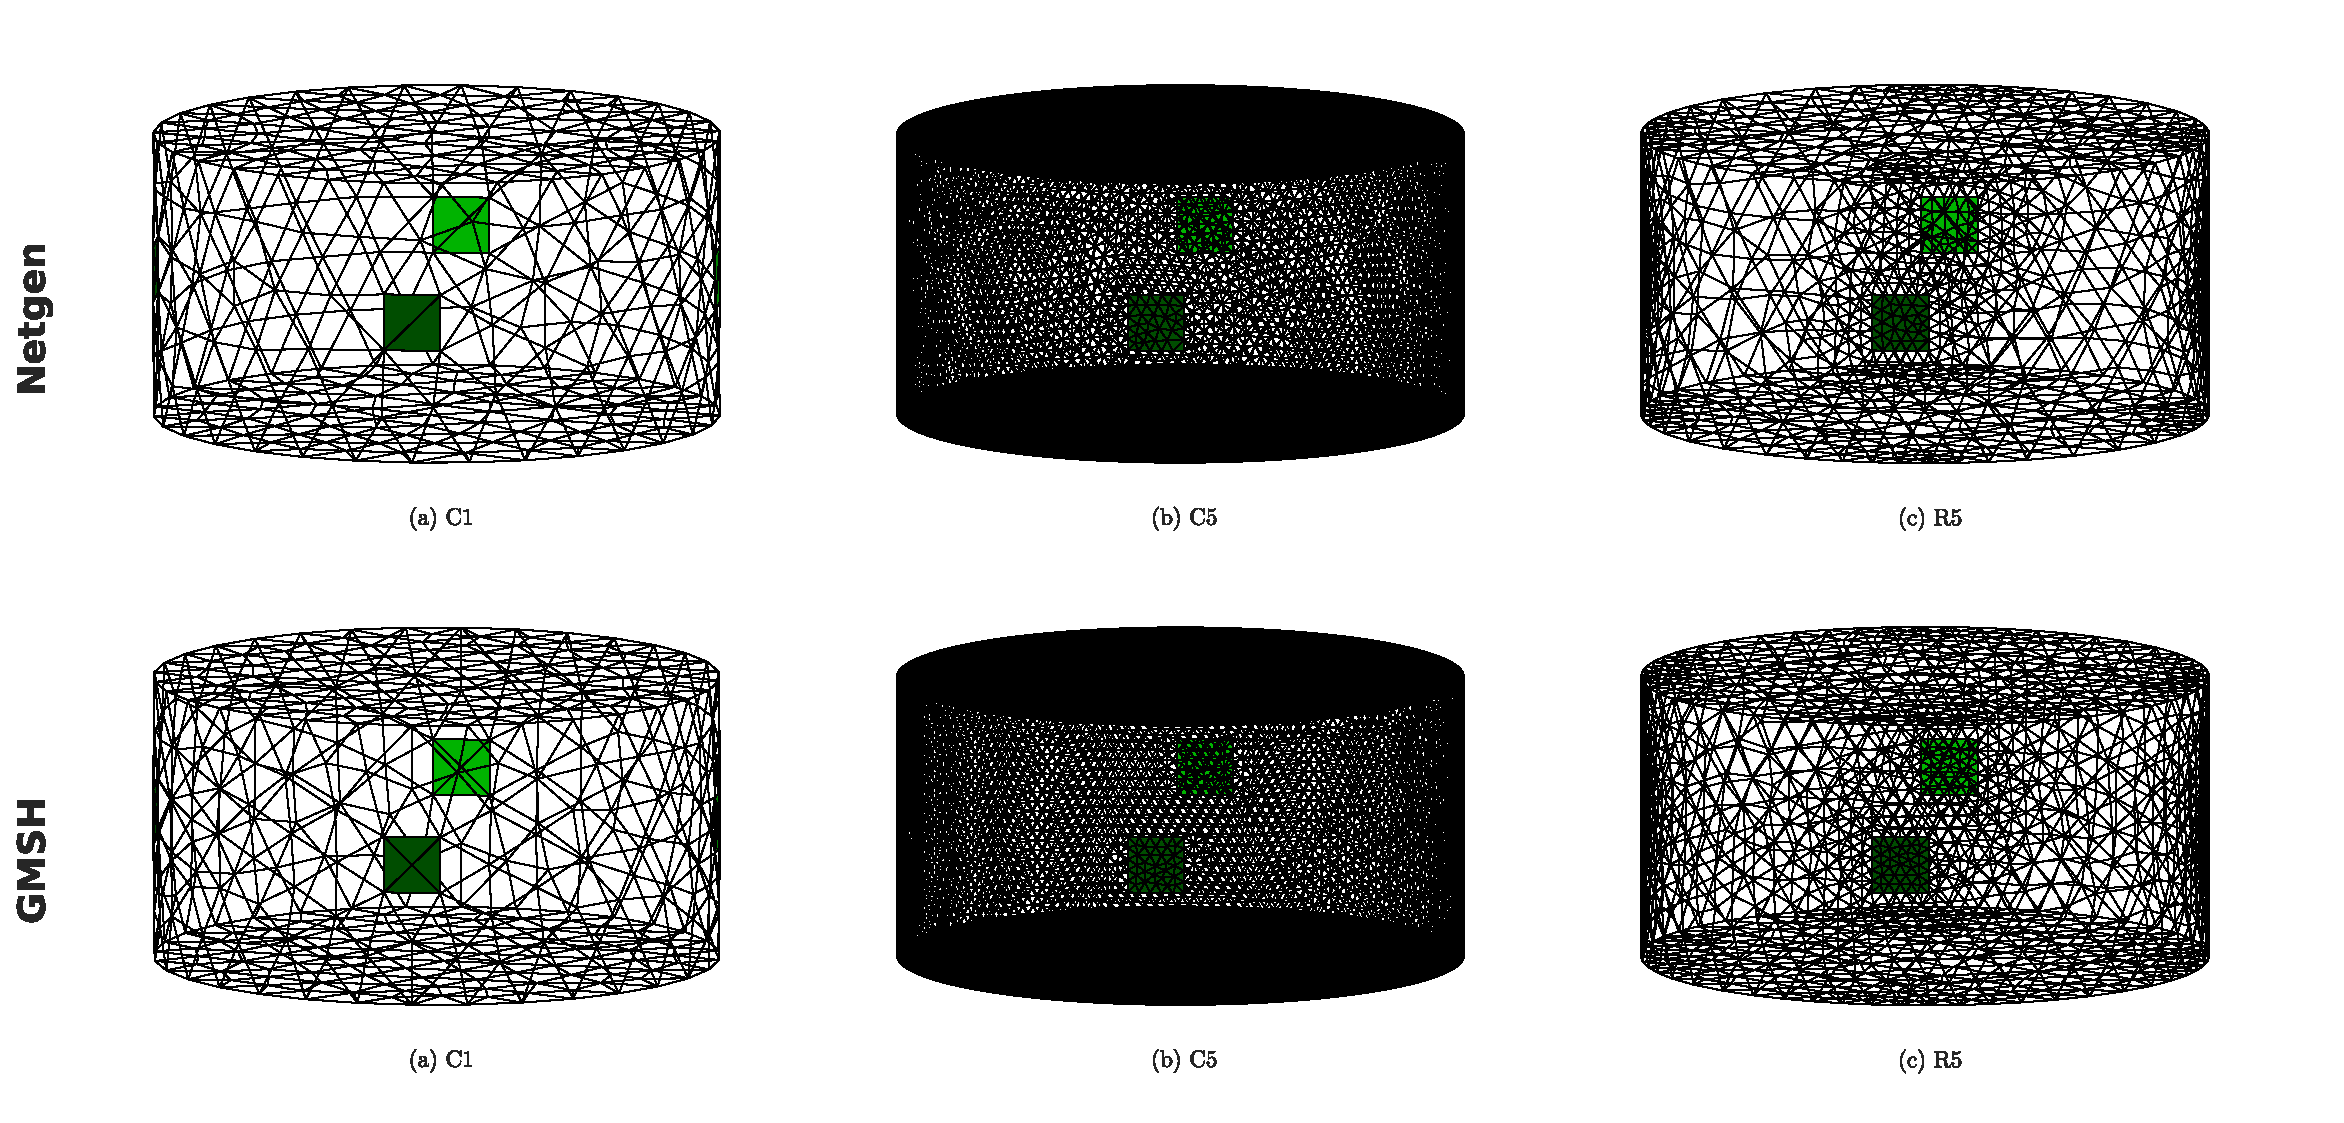
\includegraphics[width=\columnwidth]{chapter4-mesh_refinement/imgs/sample_meshes.pdf}
   \caption[Example meshes for various refinement strategies]{\label{fig:sample_meshes} 
   Sample meshes generated with Netgen (top row)
   and Gmsh (bottom row). From left to right: (C1) the coarsest constant
   mesh; (C5) a refined constant mesh; and (R5) a refined mesh with the same
   electrode mesh density as C5 but lower internal mesh density.}
\end{figure}

\begin{figure}[H]
  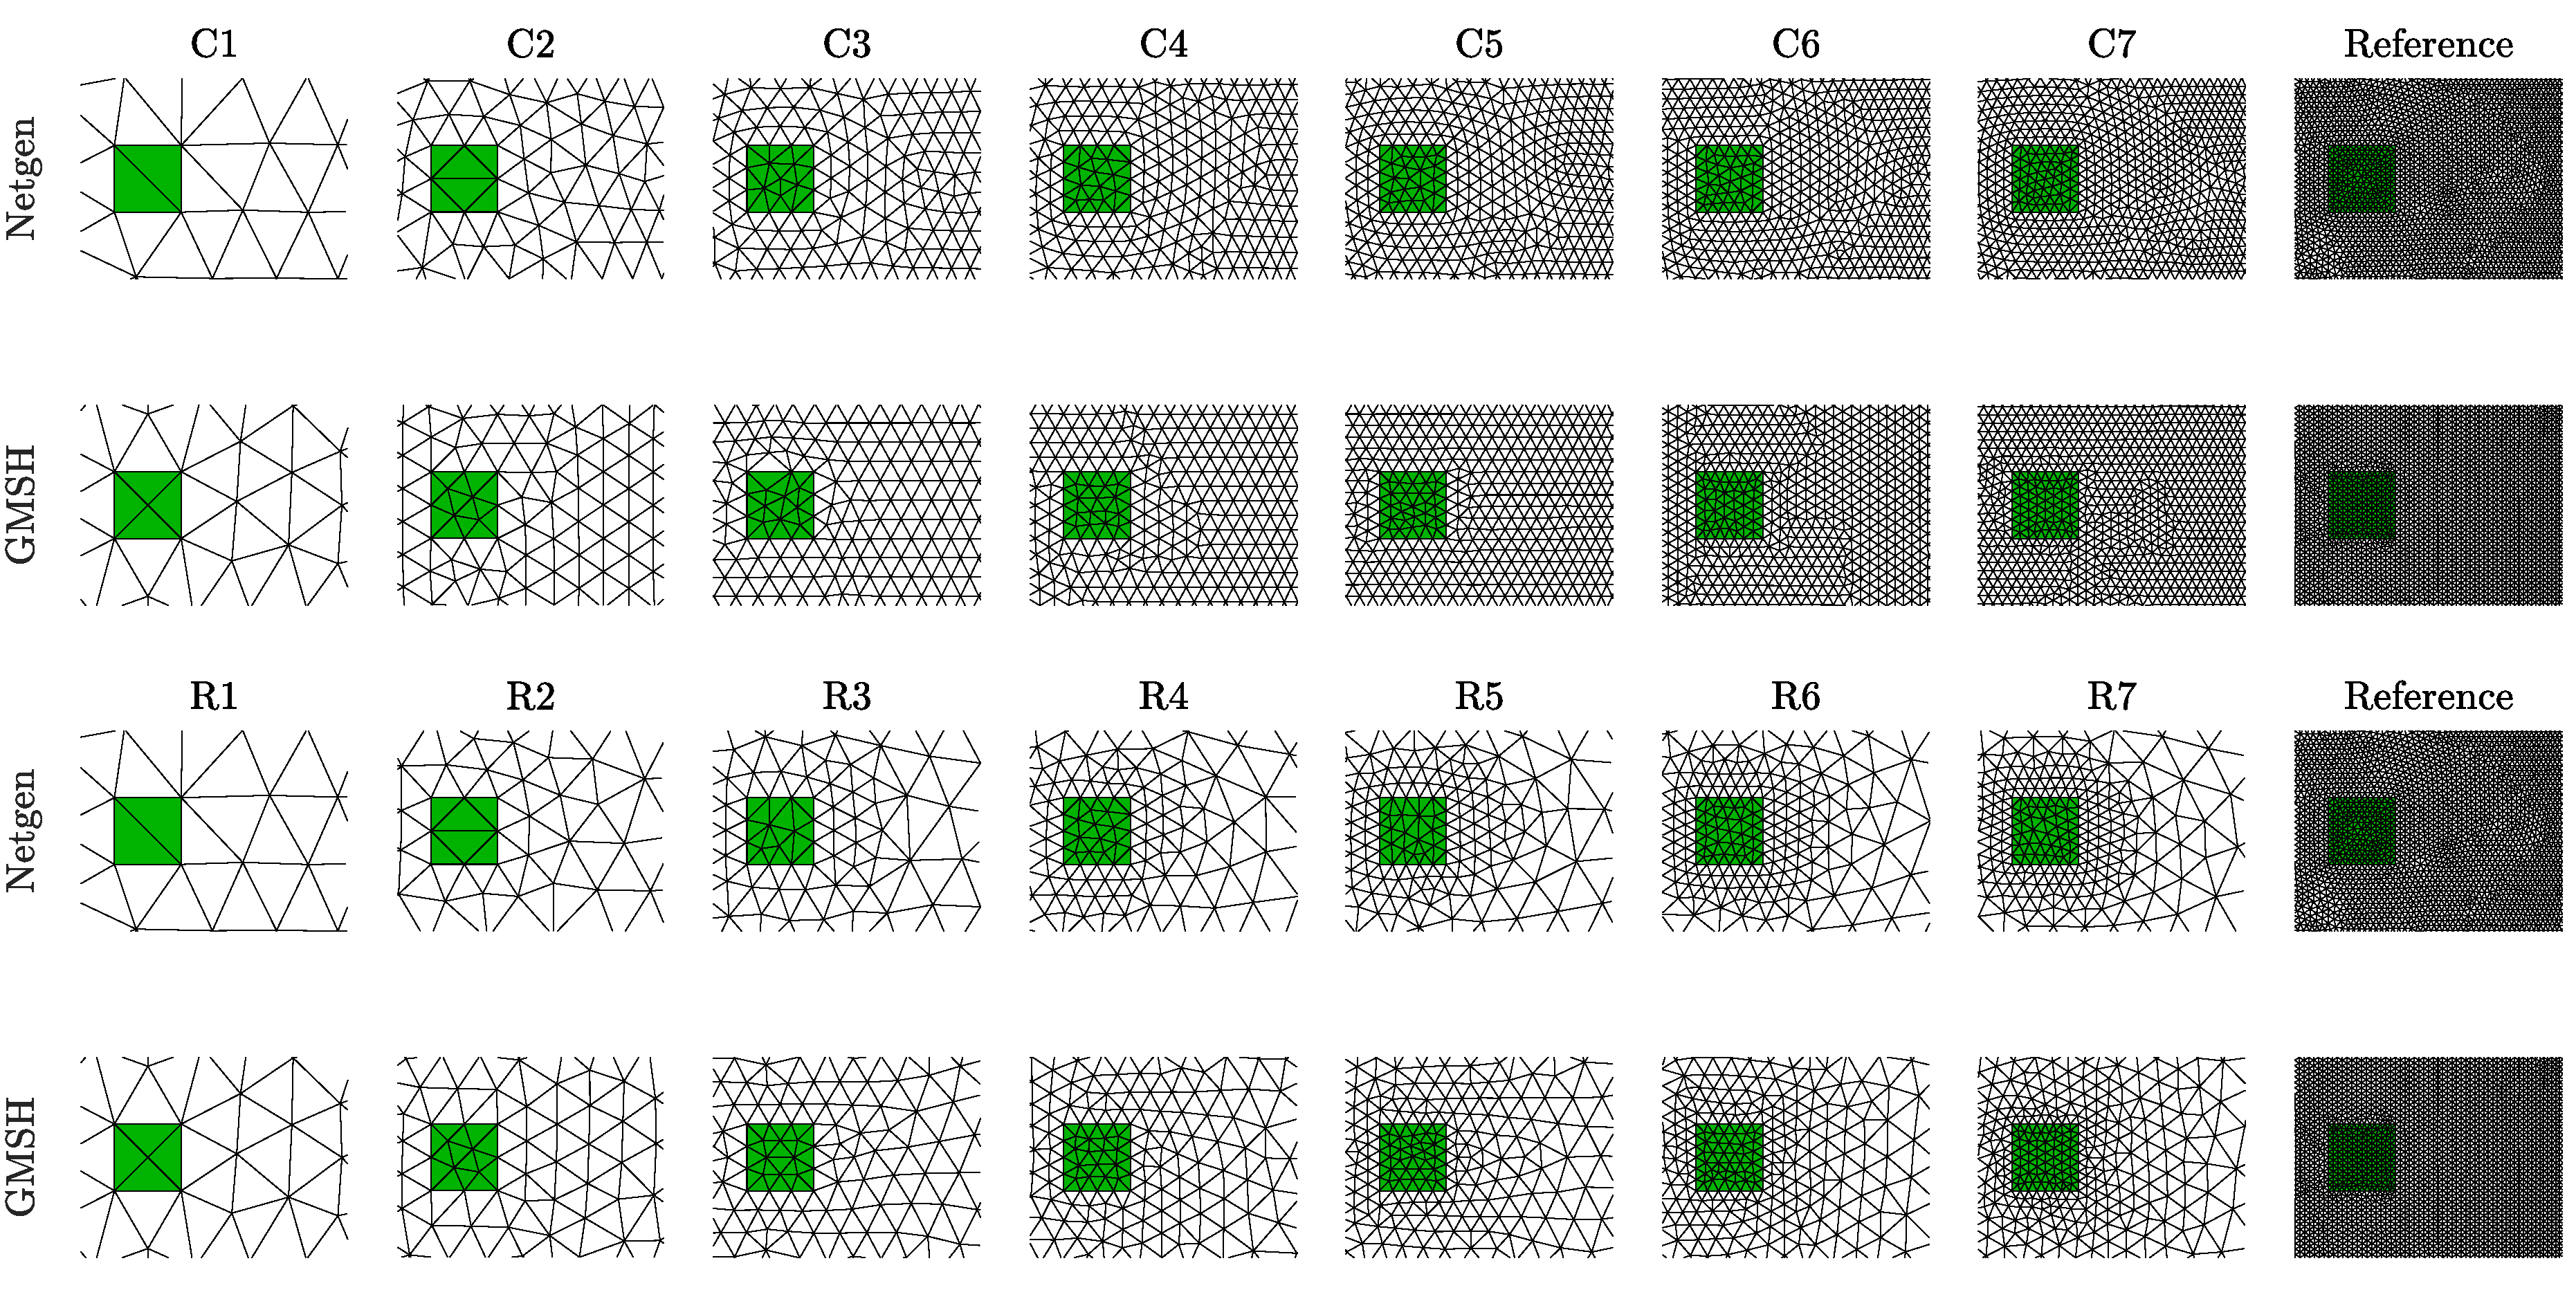
\includegraphics[width=\textwidth]{chapter4-mesh_refinement/imgs/electrode_mesh_size_large.pdf}
  \caption[Mesh size surrounding the electrode]{\label{fig:electrode_mesh_size} A view of the electrode meshing for all constant-density meshes 
  in Netgen and Gmsh. The top two rows show all electrode faces and immediate surrounding
  surroundings from coarsest (C1) to finest (C7). C represents the constant mesh refinement and the number
  represents the specified mesh subdivisions per electrode edge. The reference mesh is equivalent to C15.
  The bottom two rows show refined meshes R1 to R7 with both Netgen and Gmsh and shows the rate of mesh
  dissipation away from the electrodes.}
\end{figure}

For the second analysis, the distribution of nodes within the 
model was changed without altering 
the total number of nodes to give M1--M17. 
Starting with the constant mesh C3 as M1, the maximum mesh element 
length on the electrode was decreased by 10\% and the maximum mesh size in the centre was
increased so that the total number of elements in the mesh was  within 10\% of the 
original mesh. C3 was chosen as the starting point because several steps of mesh 
refinement could be generated before the electrode mesh density surpassed the reference meshes. 
For mesh M17 the specified electrode refinement was equal to the reference mesh. 
In Netgen the mesh dissipation rate was not further controlled, and in Gmsh the mesh density 
decreased evenly from the electrode surface to the centre of the model. 
To compare these meshes a section of the model was selected
encompassing all points between the centre of the model and a selected electrode face.
The average 
distance, or balance point, along the x-axis of the selected points was expressed 
as a percentage of the tank radius.
This process is illustrated in \fref{fig:balanceMethods}.
 
\begin{figure}[H]
  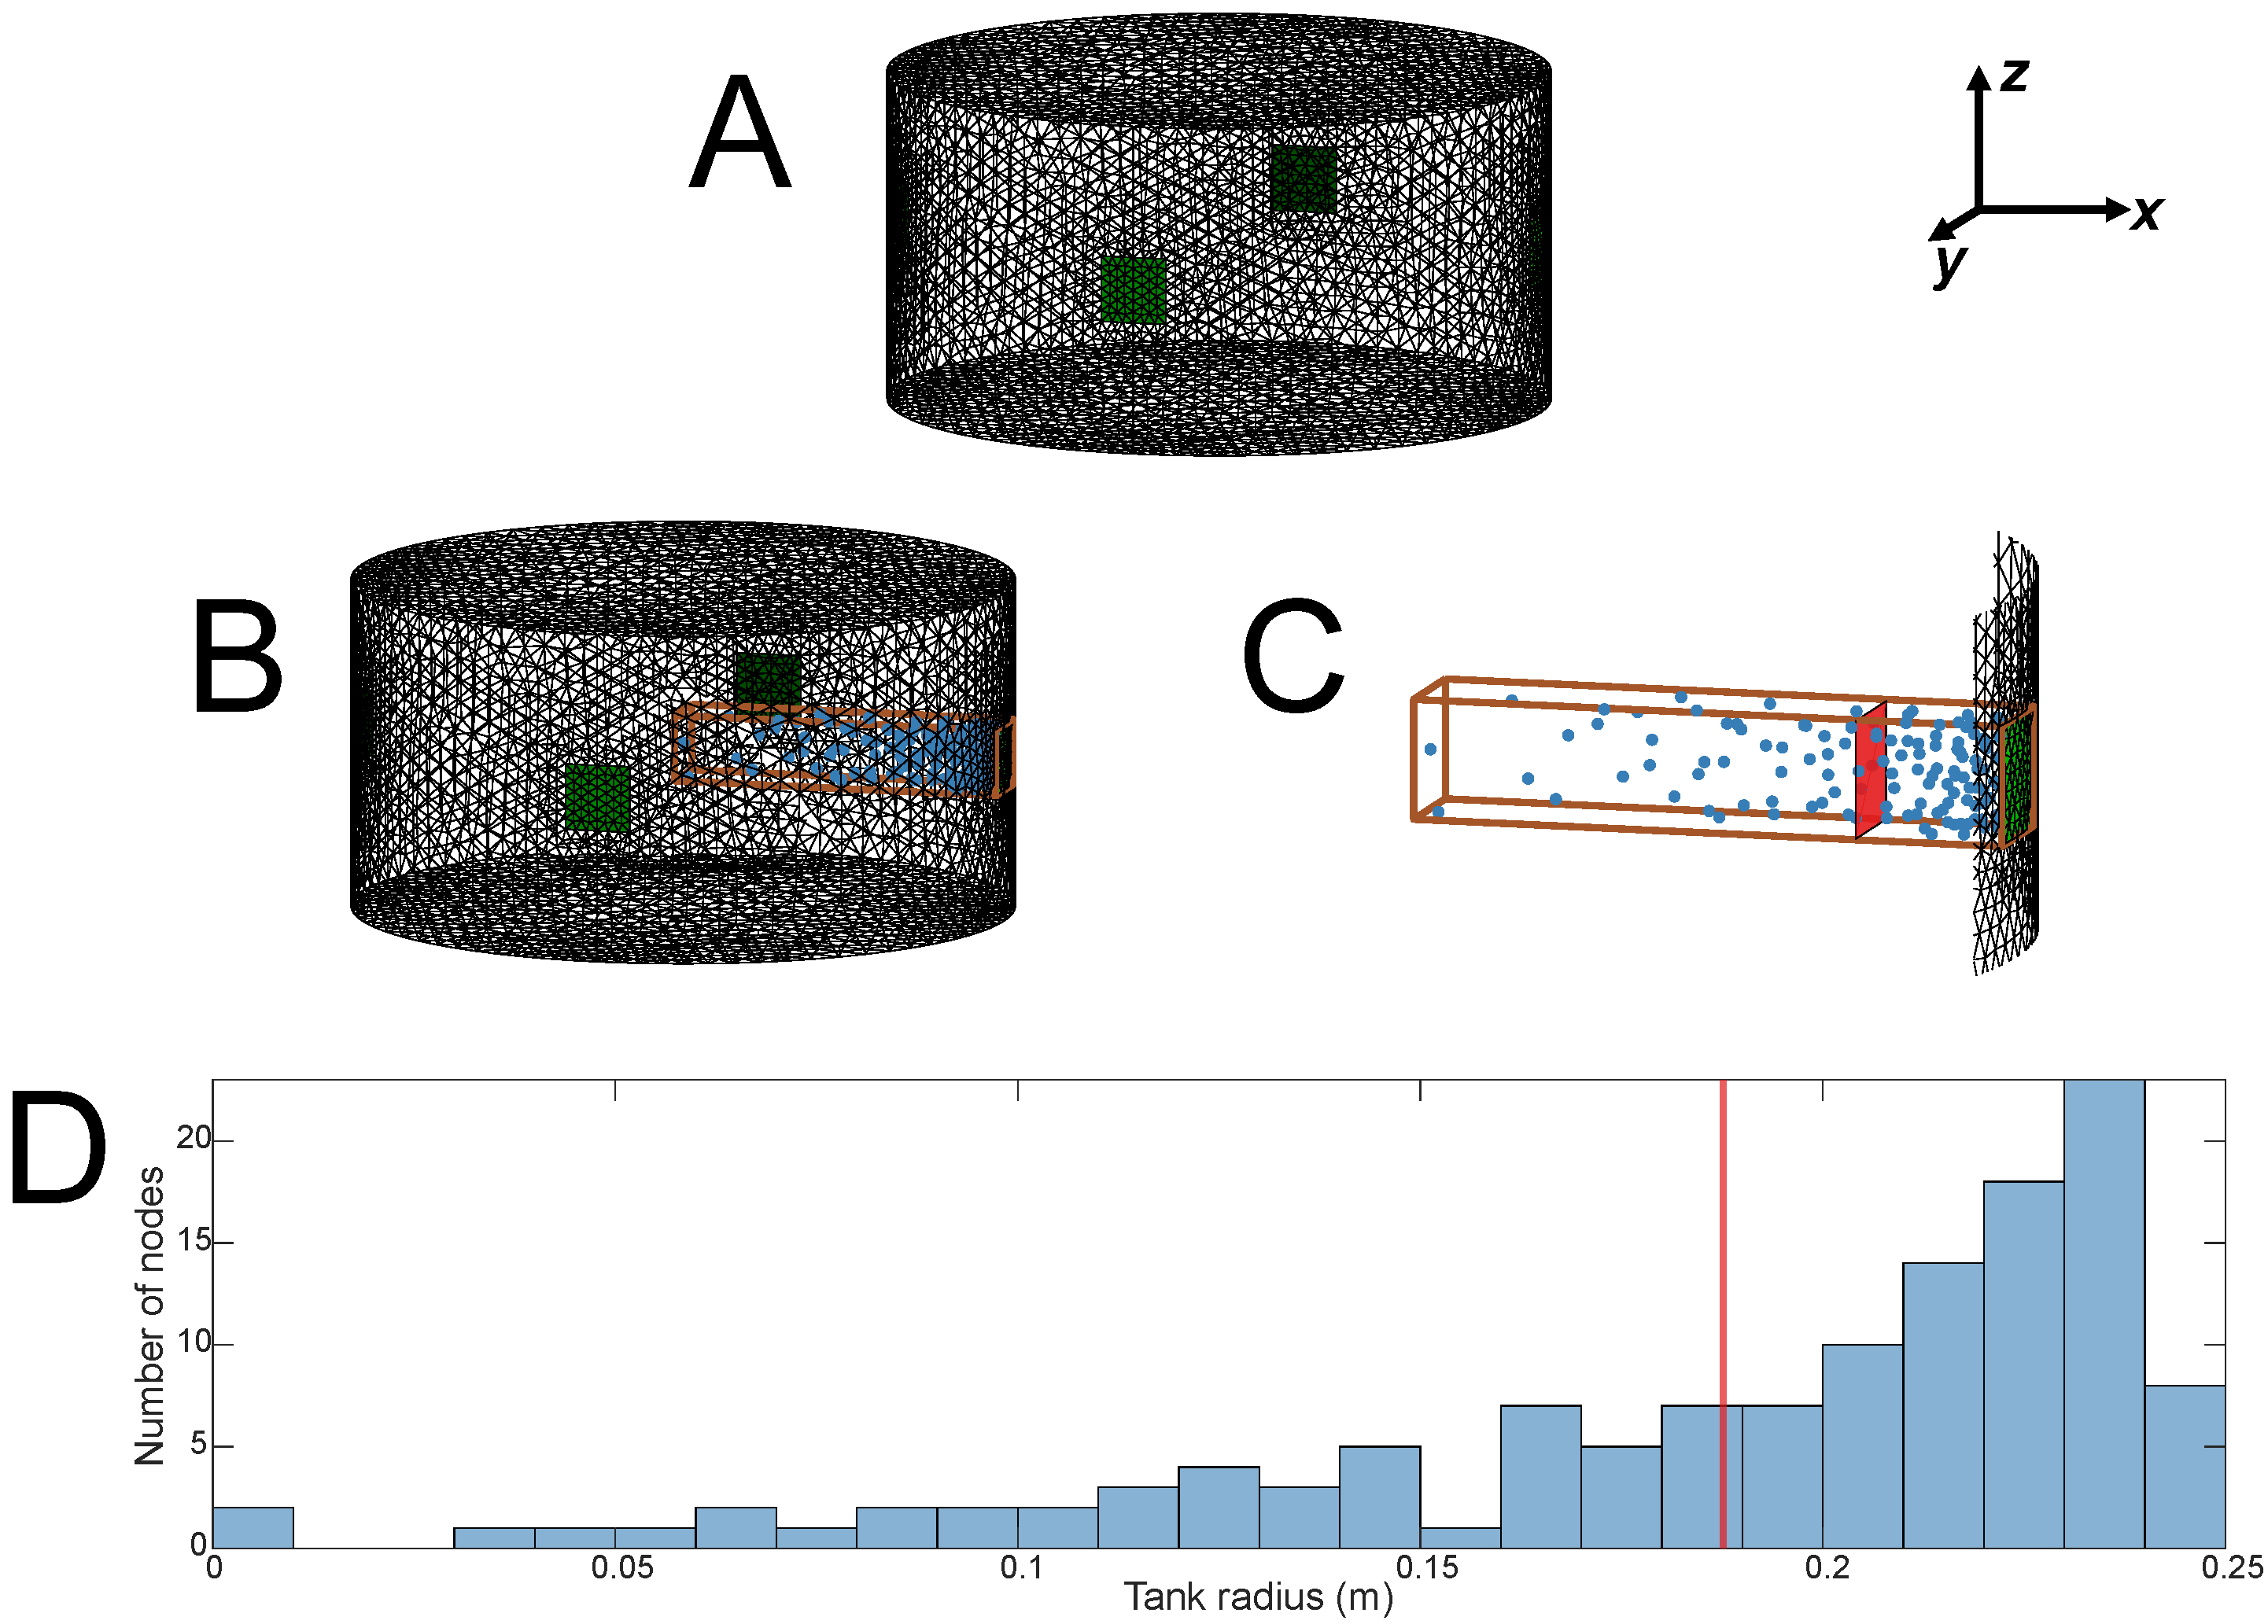
\includegraphics[width=\columnwidth]{chapter4-mesh_refinement/imgs/balance_methods.pdf}
  \caption[Balance point calculation method]{\label{fig:balanceMethods} A sketch of the process to determine the 
  balance point of generated meshes. A) the starting mesh; B) nodes between the
  electrode surface and the centre of the model are identified; C) the 
  balance point of the nodes along the x-axis is calculated and indicated 
  by the red plane; D) a histogram showing an example distribution and balance point (red)
  for the selected model.}
\end{figure}

When generating meshes to compare across several mesh density profiles as the balance of the nodes was shifted 
towards the electrodes, 19 meshes were generated for each software including 2 reference meshes. 
\Fref{tab:mesh-table} shows the parameters of the resulting odd numbered meshes. 

% Table 
\begin{table}[]
\caption[Parameters used to generate meshes]{\label{tab:mesh-table}Mesh parameters for odd numbered meshes generated by Netgen (A) and Gmsh (B) 
to determine the optimal 
node balance. Parameters global maxh and electrode maxh refer to the specified input parameters; the remaining 
columns give parameters from the resulting meshes.}
\vspace{3mm}
\resizebox{\textwidth}{!}{
\begin{tabular}{p{0.7cm}p{0.2cm}p{1cm}p{1cm}|p{1.4cm}p{1.4cm}p{1cm}|p{1.3cm}p{1.3cm}p{1.3cm}p{1.3cm}}
\multicolumn{2}{l}{Mesh ID} & glbl. maxh [mm] & elec. maxh [mm] & \#~elem. & \#~nodes & \#~elec. elem. & minEL\textsuperscript{\emph{a}} [mm] & maxEL\textsuperscript{\emph{b}} [mm] & minEV\textsuperscript{\emph{c}} [mm\textsuperscript{3}] & maxEV\textsuperscript{\emph{d}} [mm\textsuperscript{3}]\\ \hline 
\multirow{2}{*}{M-01} &A & 16.67 & 16.67 & 31347 & 7095 & 22 & 9.80 & 49.45 & 254.76 & 6851.01\\ 
& B & 16.67 & 16.67 & 49210 & 9615 & 25 & 10.32 & 50.00 & 222.87 & 2898.59\\ 
\multirow{2}{*}{M-03} &A & 18.33 & 15.00 & 29639 & 6482 & 22 & 10.75 & 50.41 & 289.80 & 5826.14\\ 
& B & 18.33 & 15.00 & 49247 & 9680 & 40 & 7.36 & 37.11 & 172.78 & 2814.55\\ 
\multirow{2}{*}{M-05} &A & 18.33 & 13.33 & 29814 & 6589 & 28 & 9.39 & 49.91 & 162.26 & 5648.41\\ 
& B & 20.00 & 13.33 & 50749 & 9930 & 42 & 7.80 & 37.93 & 134.41 & 3233.59\\ 
\multirow{2}{*}{M-07} &A & 18.33 & 11.67 & 30581 & 6723 & 36 & 8.77 & 47.88 & 141.74 & 6252.36\\ 
& B & 21.67 & 11.67 & 53002 & 10429 & 60 & 6.17 & 40.84 & 63.22 & 4077.18\\ 
\multirow{2}{*}{M-09} &A & 18.33 & 10.00 & 30690 & 6755 & 42 & 7.86 & 49.18 & 115.45 & 5496.39\\ 
& B & 23.33 & 10.00 & 56237 & 11008 & 68 & 5.82 & 43.81 & 62.88 & 4962.89\\ 
\multirow{2}{*}{M-11} &A & 18.33 & 8.33 & 31575 & 7030 & 74 & 6.05 & 50.99 & 60.06 & 6086.88\\ 
& B & 26.67 & 8.33 & 55545 & 10886 & 96 & 5.51 & 49.72 & 36.84 & 7424.70\\ 
\multirow{2}{*}{M-13} &A & 20.00 & 6.67 & 28589 & 6447 & 92 & 4.65 & 51.85 & 20.68 & 6664.11\\ 
& B & 30.83 & 6.67 & 54993 & 10825 & 148 & 4.51 & 55.36 & 20.63 & 10453.90\\ 
\multirow{2}{*}{M-15} &A & 21.67 & 5.00 & 27775 & 6245 & 158 & 3.46 & 52.60 & 11.13 & 9097.30\\ 
& B & 36.67 & 5.00 & 55331 & 11000 & 250 & 3.51 & 61.66 & 7.99 & 15838.09\\ 
\multirow{2}{*}{M-17} &A & 30.00 & 3.33 & 39116 & 7590 & 320 & 1.75 & 72.83 & 1.13 & 23783.17\\ 
& B & 48.33 & 3.33 & 52947 & 10798 & 548 & 2.32 & 86.60 & 2.72 & 32287.34\\ \hline 
\multirow{2}{*}{REF} &A & 3.33 & 3.33 & 6661789 & 1173243 & 510 & 1.75 & 9.49 & 1.01 & 46.09\\ 
& B & 3.33 & 3.33 & 5871464 & 976558 & 554 & 2.10 & 7.59 & 1.58 & 21.65\\ 
\multicolumn{11}{c}{\emph{a}: minimum mesh edge length, \emph{b}: maximum mesh edge length}\\ 
\multicolumn{11}{c}{\emph{c}: minimum mesh element volume, \emph{d}: maximum mesh element volume}\\ 
\end{tabular}
}
\end{table}

%The difference in meshing algorithms meant that the meshes did not have the same number
%of elements, or elements per electrode for a given input. To compare meshing 
%algorithms the error and sensitivity were compared to the average number of mesh elements\
%across all electrodes. 
%
%
%%The settings used to generate all thirty meshes and their sizes are reported
%%in Table~\ref{tab:meshes}. 
%%{\COMMENT{Broke table with new analysis - need to re-insert after electrode mesh fix.}}
%
%The mesh quality was measured as a function of the minimum angle of the tetrahedra
%for the volumetric mesh, and the minimum angle of the triangles in the surface mesh.

\subsection{Simulation}
%The potential at each node \VB\ of the mesh was calculated using the finite
%element method (FEM) using the linearization 
%\begin{equation}
%\VB = \YB^{-1}\CB
%\end{equation}
%where \YB\ is the admittance matrix of the FEM (and a function of conductivity
%distribution) and \CB\ is a matrix representing the current injection pattern,
%such that \CB$_{ij}$ represents the current injected in electrode $i$ during
%the $j$-th stimulation. Here, we drive current of 1~A between two adjacent
%electrodes in a single stimulation, so $C = [0\,|\,0\,|\,1\,|\,-1]^T$. 
%We pick a node in the centre of the FEM as ground, since it is necessary to
%assume the potential on
%one node for \YB\ to be invertible.
%We use the complete electrode model and assume contact impedance of
%0.01~$\Omega$ in the calculation of the admittance
%matrix~\parencite{polydorides_electrode_2002}. 

%The resultant potential distribution in the
%electrode plane, calculated for the finest mesh and subsequently projected onto
%a $512\times512$ pixel grid, is presented in Fig.~\ref{fig:ref:a}.
%The potential distribution \VB\ is used to visualize the current flow
%around the measuring electrodes.
% NOT CURRENTLY LOOKING AT THE CURRENT FLOW! seems to be a repeat of the same stuff
To calculate the sensitivity of each measurement to a change in conductivity of each element
we use the adjoint method \parencite{polydorides_electrode_2002}. 
\begin{equation}
  \JB_{ij}=\frac{\partial v_j}{\partial \sigma_i}
\end{equation}
A sensitivity was normalized by dividing the sensitivity value for each element 
by the element's volume. 
The average sensitivity of 15 planes evenly spaced between the top and bottom edges of the electrodes
was used to generate a sensitivity image.
%We calculate the sensitivity (or Jacobian) matrix \JB\ of measurements \vB\ to
%changes in the conductivity $\sigma$ of individual elements as
%$\JB_{ij}=\frac{\partial v_j}{\partial \sigma_i}$ using the adjoint
%method~\parencite{polydorides_electrode_2002}. Again, since we only have one measurement, \JB\
%is in fact a vector.
%We construct a sensitivity image by assigning each element
%$i$ of the FEM the value of \JB$_i$ divided by the element's volume.
%Mean sensitivity in the plane of electrodes is then calculated by averaging
%the sensitivity in fifteen planes parallel to the plane of electrodes and
%spanning the height of 5~cm. 
The EIT image structure was rasterized onto a $512\times512$ array, and divided into 3 regions of interest:
%The sensitivity was projected onto a $512\times512$ array and divided into regions
%of interest for 
the centre of the model (C), adjacent to the electrode (E) and between the centre and electrode
(I). The resulting sensitivity for the reference mesh calculated with Gmsh and the 
selected regions of interest are presented in \fref{fig:roiMethods}.

To calculate the sensitivity error, the difference in sensitivity wasa computed between the 
reference model and the refoned models to give the total error in sensitivity.
The normalized sensitivity error is calculated as the absolute sensitivity error 
divided by the total sensitivity error
for the selected region.

%\subsection{Meshing errors}
%We compare the meshes in terms of the value of the voltage measurement between
%the non-stimulating electrodes, and the mesh quality as determined by the minimum 
%angle in the tetrahedral elements.
% %the distribution of current around the measuring
%%electrodes and the average sensitivity in select regions of interest (ROI) in
%%the electrode plane. 
%%The ROIs are indicated in Fig.~\ref{fig:ref:a}. 
%We use the results obtained
%with the C0 mesh as reference to compare the others against.

\subsection{Electrode Refinement for Arbitrary FEMs}
Our approach for refinement around electrodes in Gmsh with external electrodes 
also allows for the refinement of arbitrary models with complex structures
such as internal electrodes and tissue boundaries.
A scenario depicting an approximation of 
a probe entering a bone with different 
layers of conductivity was modelled. The resulting mesh pictured in 
\fref{fig:adv_mesh}
highlights the ability of this technique
to be used for refinement around electrodes and the control of mesh density  
surrounding internal structures which was previously
very challenging in EIT software.

\section{Results}

Two analyses of mesh refinement were completed. First, comparing normalized sensitivity error between
meshes with constant refinement and refinement only at the electrodes; Second,
comparing meshes with different levels of electrode refinement and the same number of nodes.

When comparing constant meshes to meshes with refinement at the electrodes only, 
normalized sensitivity error
was decreased as more nodes were added to the mesh and to the electrodes. The sensitivity
error was lowest in the constant meshes across both Netgen and Gmsh software. Meshes 
generated using Netgen
provided a slightly lower sensitivity error relative to the respective reference mesh
compared to Gmsh, and resulted in meshes with fewer nodes per electrode given the same input
parameters. \fref{fig:results_sens_original} shows the sensitivity error between
constant and refined meshes with respect to the number of nodes per electrode.  

\begin{figure}[H]
  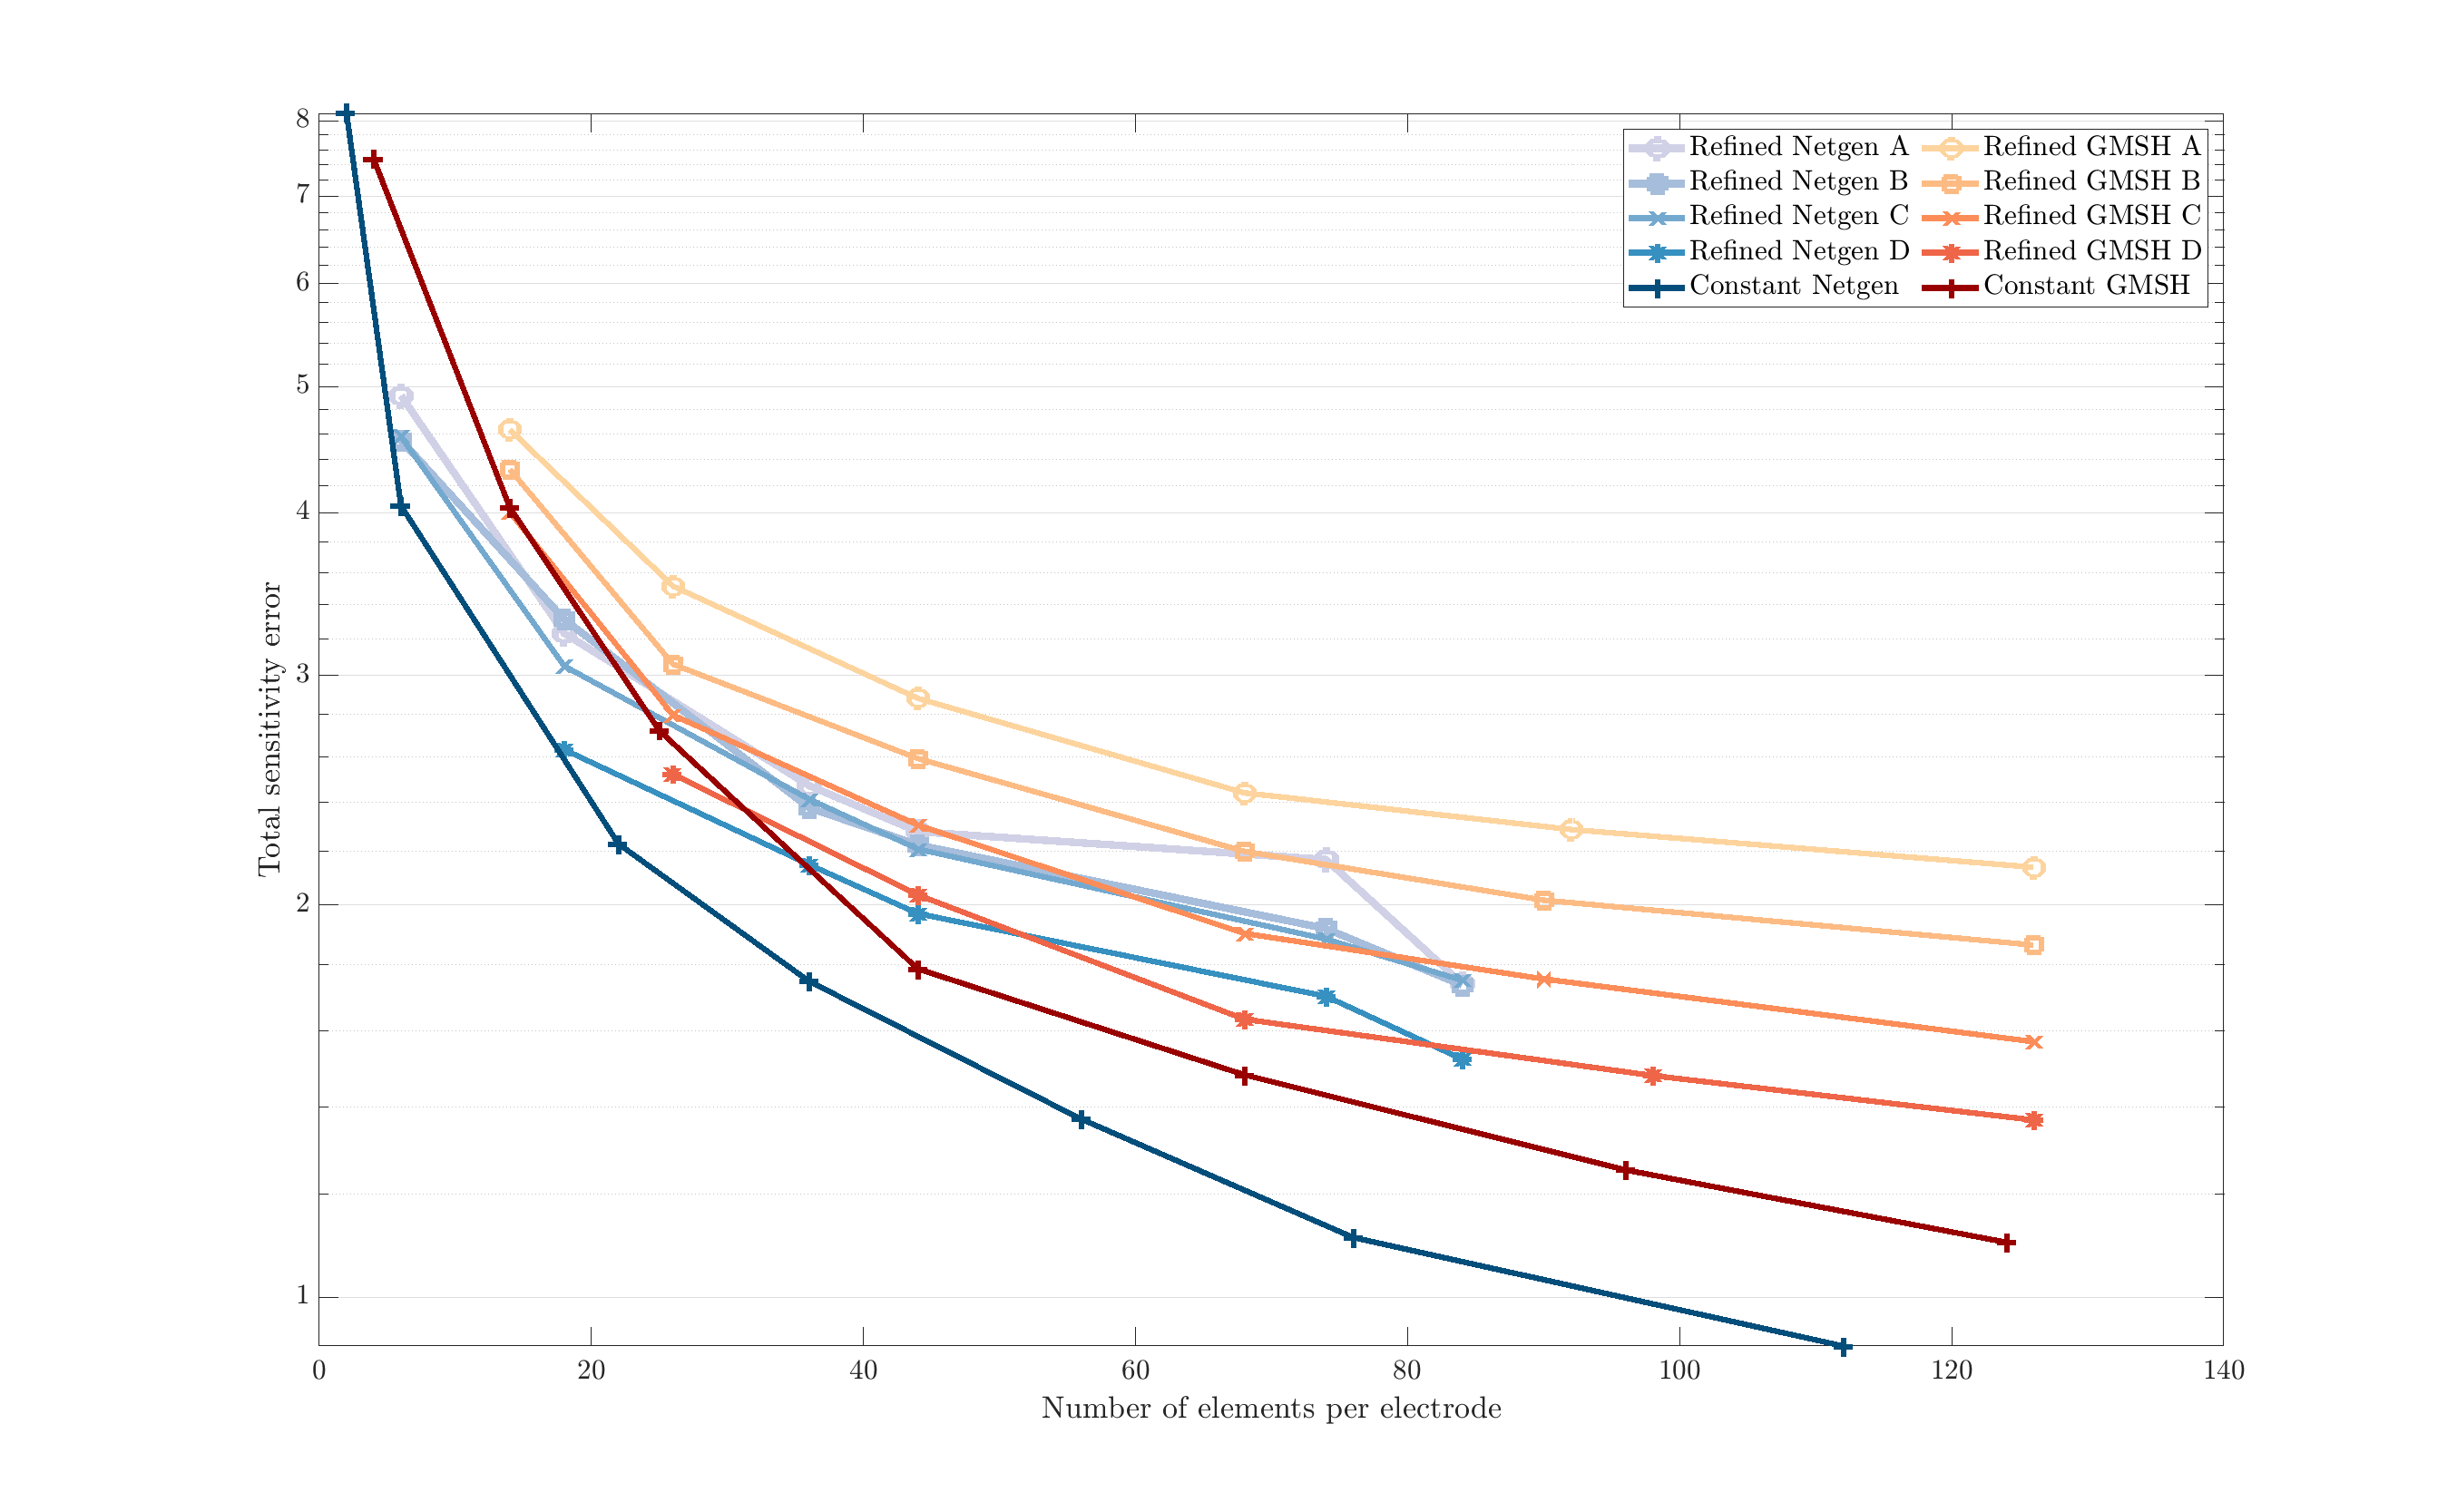
\includegraphics[width=\columnwidth]{chapter4-mesh_refinement/imgs/sens_error_total.pdf}
  \caption[Mesh sensitivity error vs. elements per electrode]{\label{fig:results_sens_original} 
  Normalized sensitivity error of each mesh as a function 
  of the number of elements per electrode for both Netgen and Gmsh. The darkest lines indicate the
  constant mesh refinement, lighter lines indicate a larger maximum internal mesh size. The maximum
  internal mesh sizes are as follows: refinement A - 5 cm; refinement B - 4 cm; refinement C - 3 cm;
  refinement D - 2 cm.}
\end{figure}

Example sensitivity profiles for the M-series meshes are shown in \fref{fig:roiMethods}.
The resulting sensitivity profile near the electrodes more closely matched the reference case 
when refinement at the electrodes was higher. 

\begin{figure}[H]
  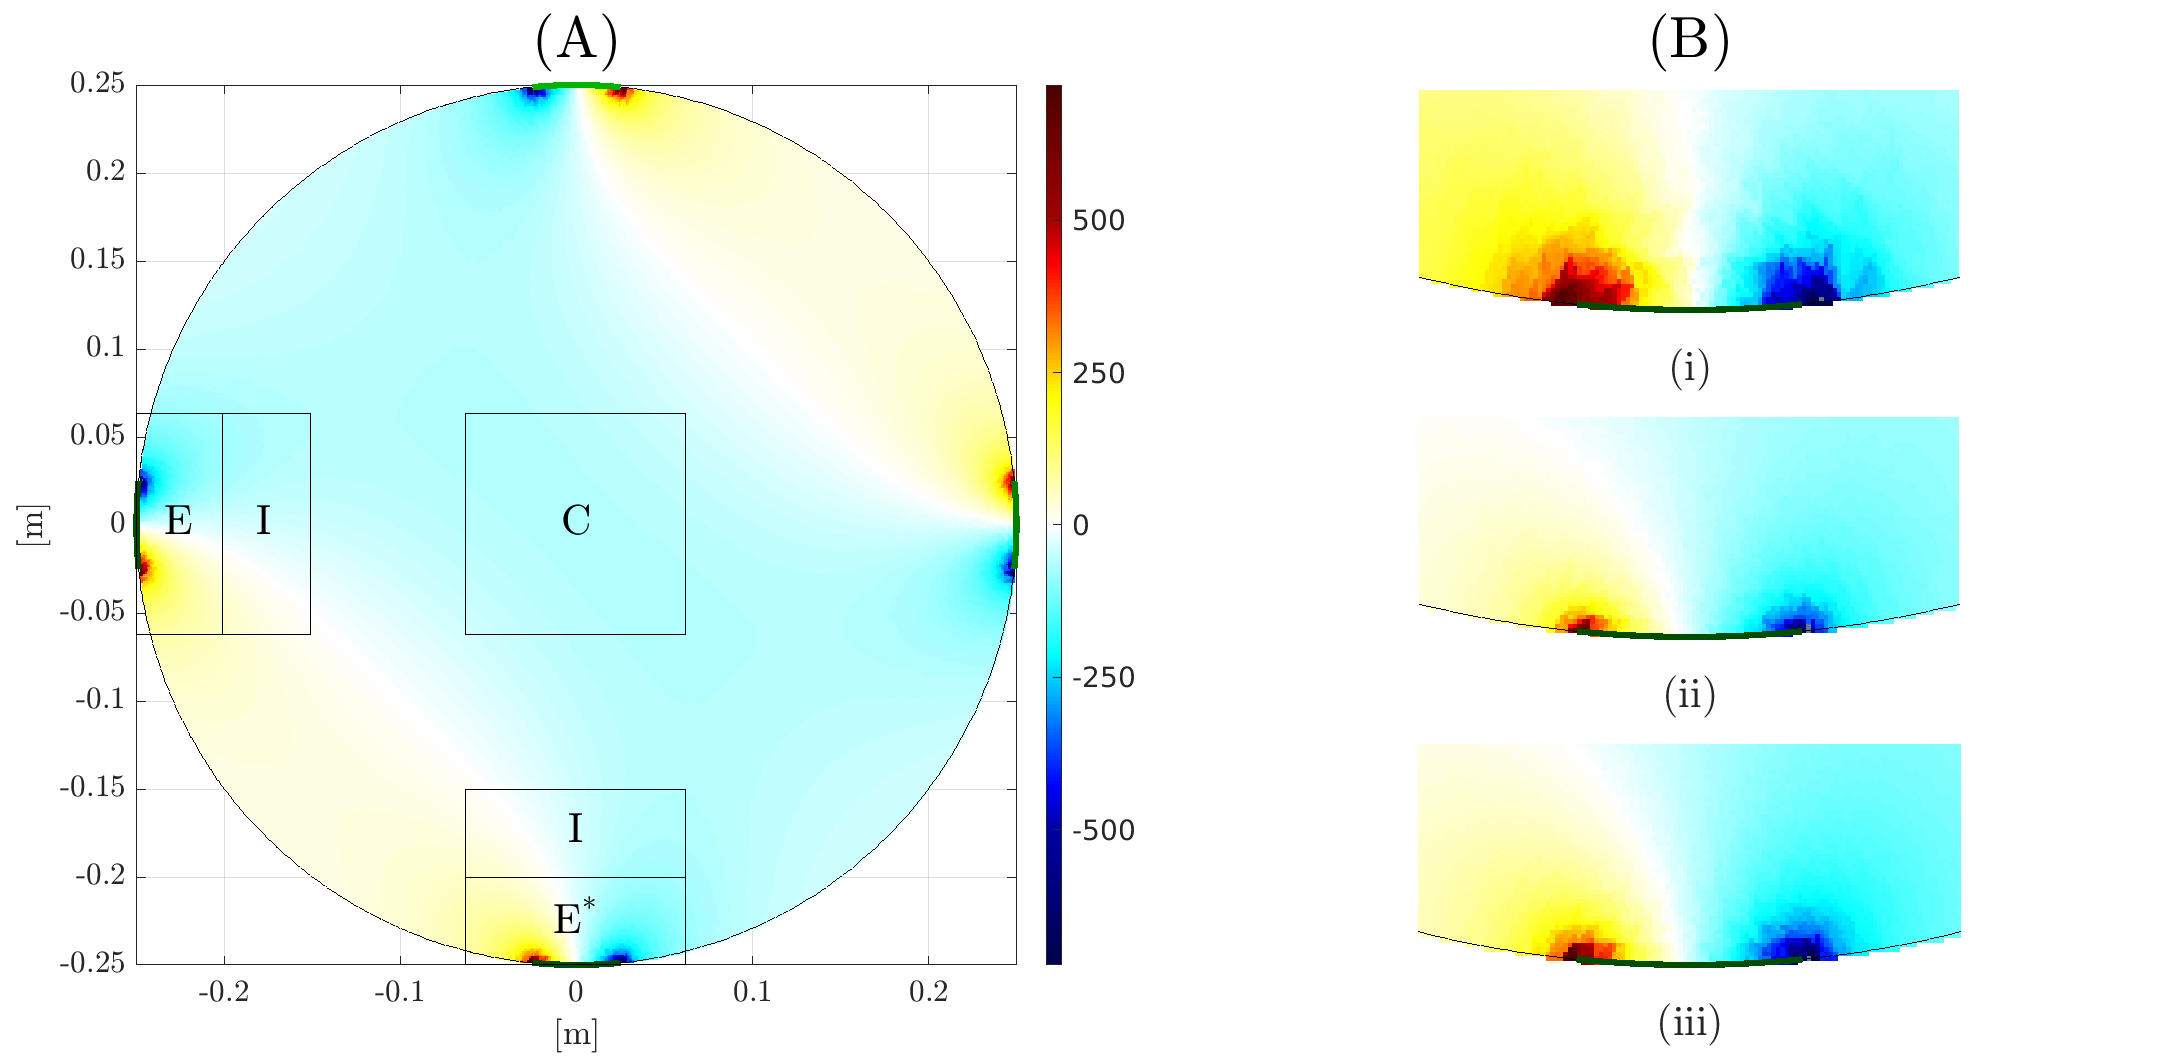
\includegraphics[width=\columnwidth]{chapter4-mesh_refinement/imgs/roi_methods_figure.pdf}
  \caption[Sensitivity distribution and regions of interest]{\label{fig:roiMethods} (A) Sensitivity distribution for the reference mesh
  (C15) generated in Gmsh with regions of interest used to compare between models. 
  (B) 3 sensitivity distributions in region E\textsuperscript{*} next to the electrodes: (i) Constant mesh M1
  (ii) refined mesh M15 with a balance point of 82\% (iii) reference mesh from (A).
  }
\end{figure}

The total sensitivity error across all meshes is plotted vs. the balance point in
\fref{fig:balance_sens}. For meshes generated with Gmsh the minimum error was 
achieved when the node balance point was approximately 85\% of the model radius corresponding
to model M15-B. 
For Netgen generated meshes the minimum sensitivity was achieved in model M13-A at a balance point
of approximately 70\%. Gmsh achieved a lower sensitivity error measured against
the respective reference mesh. For meshes using Netgen refinement, the balance point did not
increase evenly as the electrode density was increased and the internal density decreased. 
To maintain the same number of nodes within the model, Gmsh required a larger internal maxh
than Netgen. Gmsh generated meshes with more nodes for the same input
parameters, but  generally the resulting mesh sizes were closer to those specified. The
resulting mesh parameters for odd numbered meshes can be seen in \fref{tab:mesh-table}.
Across all meshes the measurement error when computing the voltage measurements was insignificant
at less than 0.2\%.

\begin{figure}[H]
  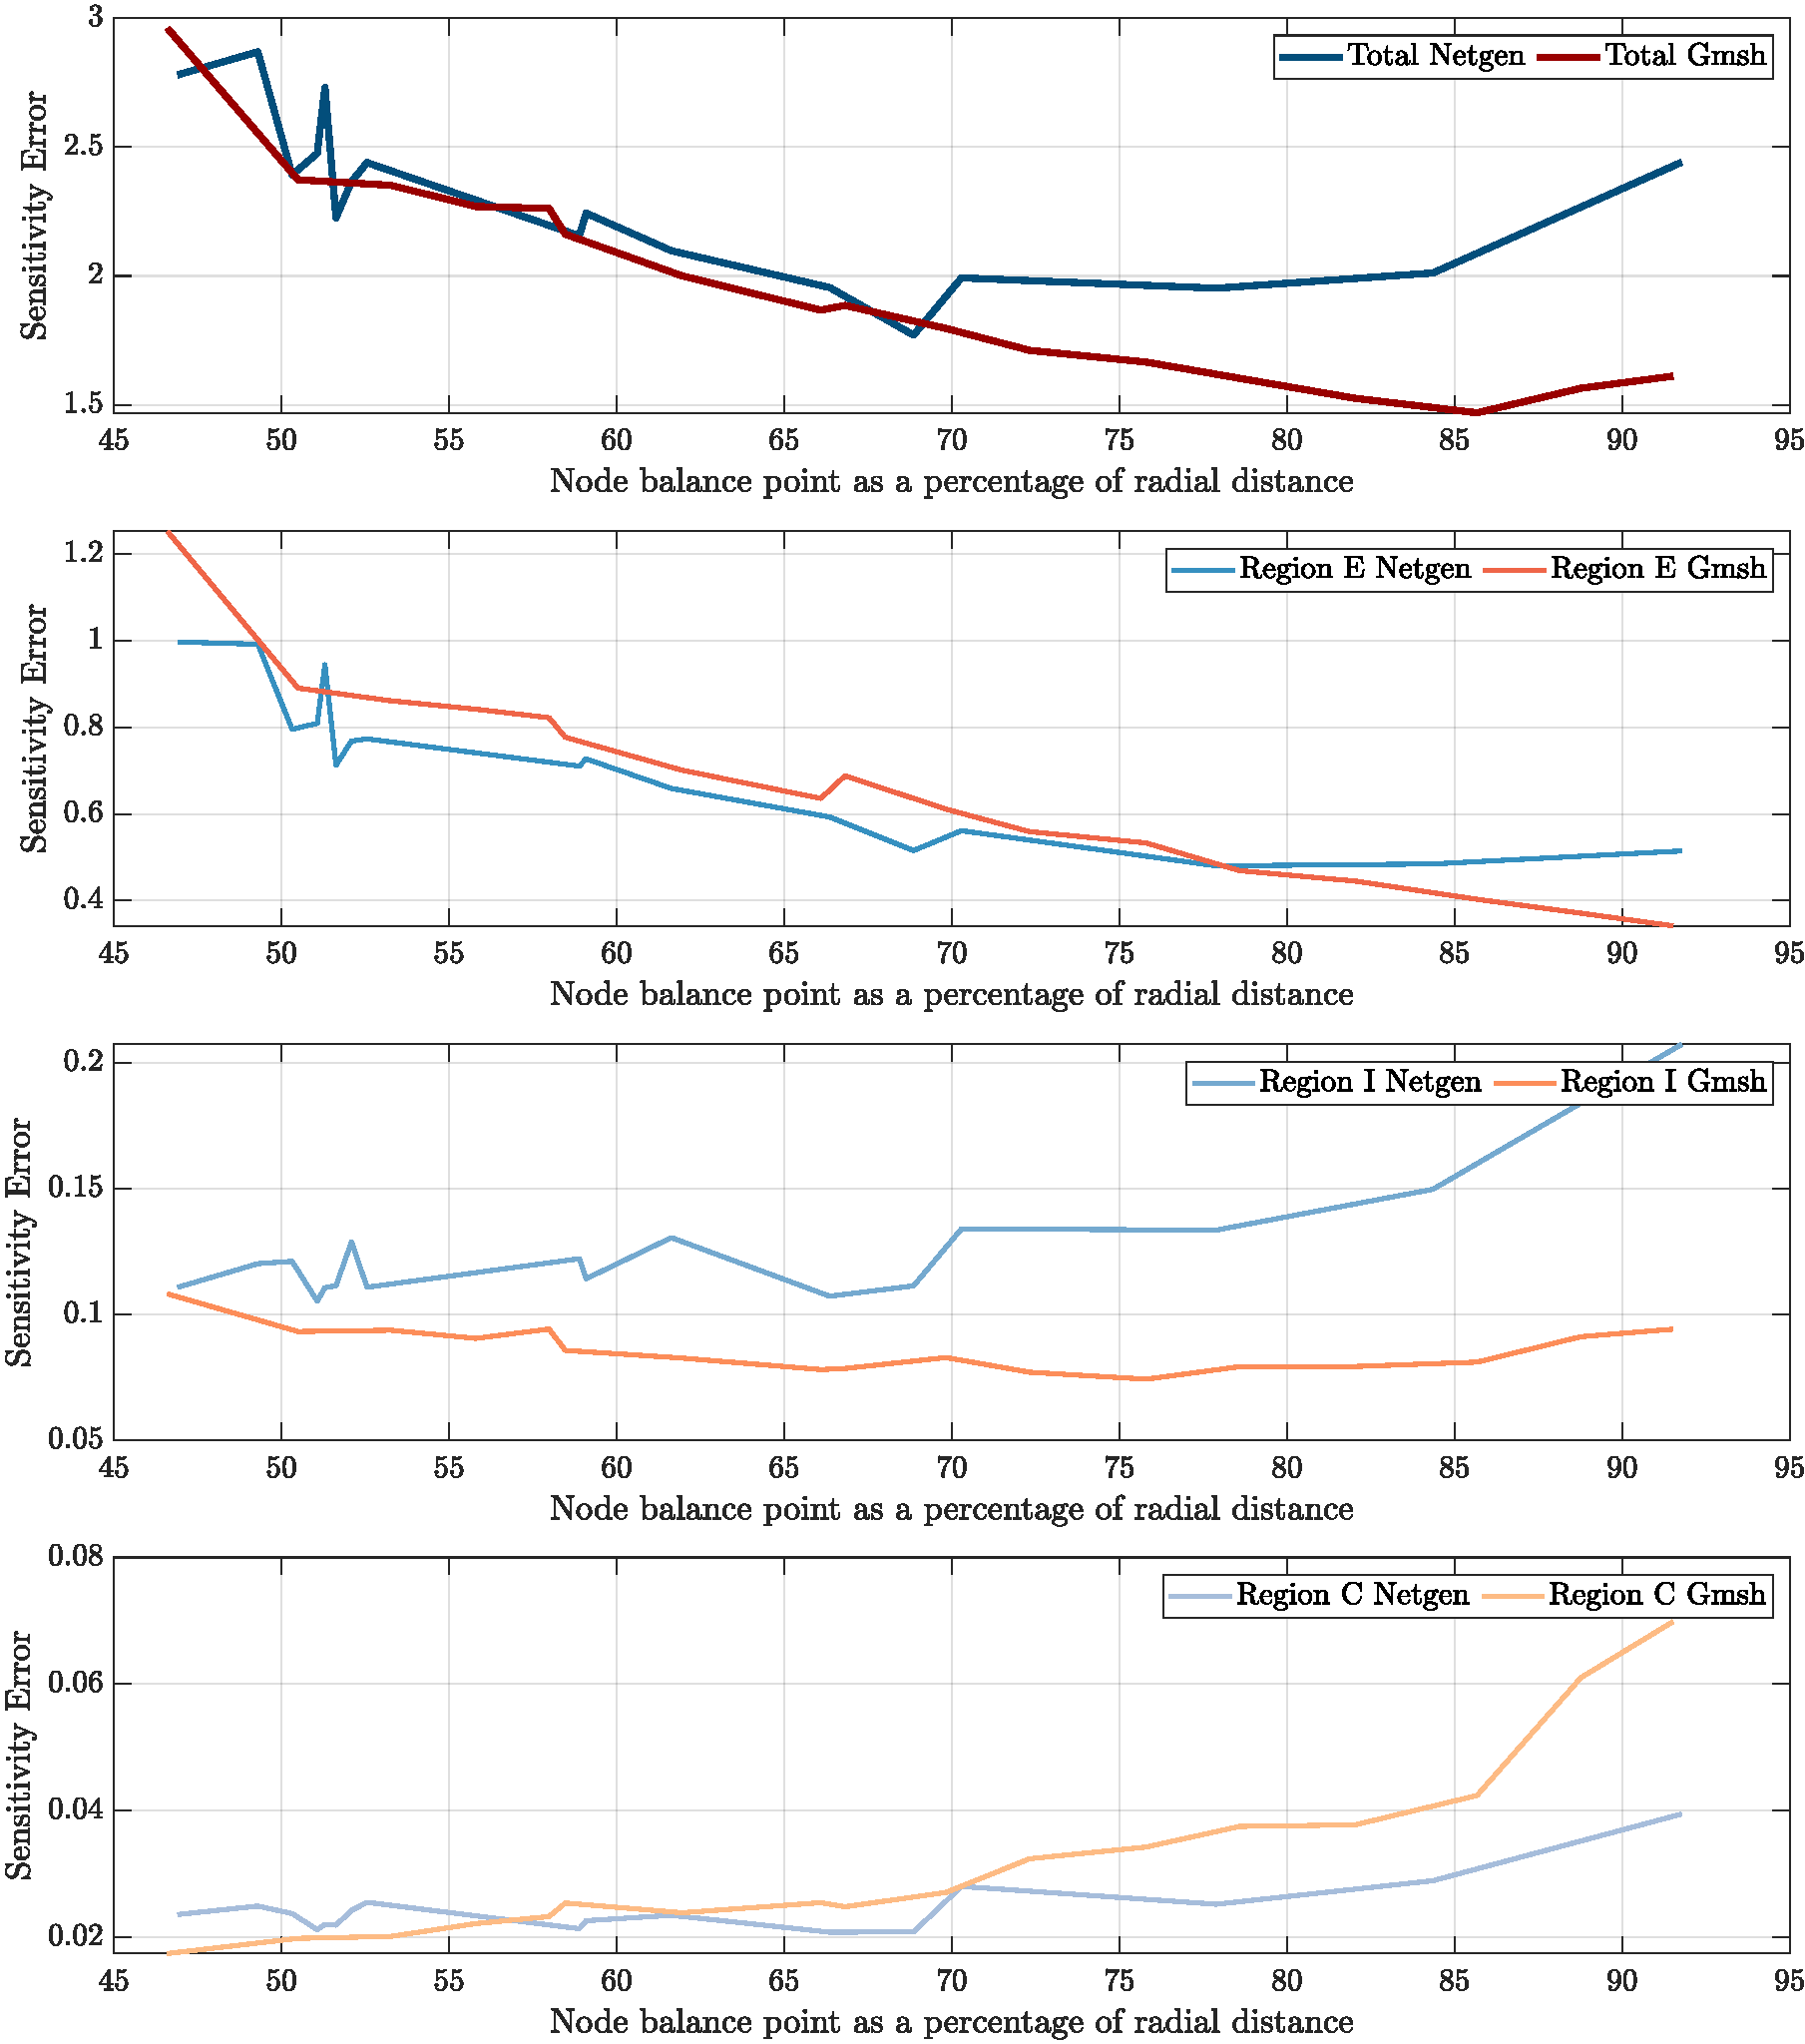
\includegraphics[width=\columnwidth]{chapter4-mesh_refinement/imgs/m-mesh_sens_error_regions_split.pdf}
  \caption[Sensitivity error with shifting node balance]{\label{fig:balance_sens}
  Resulting sensitivity error for Netgen (blue) and Gmsh (red) as the balance of the nodes
  was shifted towards the electrodes. From top to bottom: total sensitivity error, the sum of 
  sensitivity error in region E, the sum of sensitivity error in region I and the sum of
  sensitivity error in region C. The regions are described in \fref{fig:roiMethods}.}
\end{figure}

  
%  Results show that for both Netgen and Gmsh there is a significant decrease in measurement error 
%  as the number of elements throughout the model is increased. This is shown in Fig.~\ref{fig:results_meas} 
%  where the measurement error on refined meshes decreases as the models are generated with a higher 
%  density of elements. 
%  
%  For both Netgen and Gmsh when using mesh refinement techniques there was no change in the measurement error when compared to 
%  the coarsest models. % THIS DOES NOT MATCH EARLIER RESULTS WHAT IS GOING ON NOW?!?!
%  
%  When comparing mech quality based on the average minimum angle in the tetrahedra, Netgen was shown to have a higher 
%  quality mesh for constant models, but when using refinement Gmsh meshes had a better overall minimum angle score. 
%  These results are presented in Fig.~\ref{fig:results_qual} 
  
\section{Discussion}

We consider several questions on the requirement of FEM refinement near
electrodes and the available tools for mesh refinement in EIT. 
1) Given a ``FEM element budget'', what should
balance of nodes be between the centre of the model and the electrodes?
2) How do different freely available meshing tools that are
commonly used with EIT compare when used to refine 3D meshes?

While refining meshes surrounding the electrodes  is agreed to be useful,
there is a lack of systematic analysis of
the required refinement level, and controlling such
refinement is difficult. Automatic mesh refinement is an area of active work and there are
a number of commercial and free products available. We compare two programs 
used widely in EIT.
Our results show that Netgen and Gmsh control mesh refinement differently 
and the same input parameters result in meshes with different numbers of nodes. 
\fref{fig:electrode_mesh_size}, depicts the difference in
mesh dissipation rates between Netgen and Gmsh. The mesh size in Gmsh increased
gradually from the surface of the electrode  towards the centre of the model,
whereas the mesh size in Netgen increased much more quickly from the edges of the
electrode. While we attempted to control the dissipation rate in 
Netgen by manipulating the mesh density in the centre of the model, we were unable 
to achieve a smooth transition between the electrode and internal regions of the mesh. 

To analyze the benefit of electrode refinement and the difference between 
Netgen and Gmsh refinement techniques we consider
a sequence of refined meshes compared to a ``gold standard'', uniformly fine
FEM solution. The models were refined either globally or from the electrode surface, 
and the error in the sensitivity matrix $\bf J$ 
%voltage measurement,  and mesh quality %current distribution and sensitivity
was compared. \fref{fig:results_sens_original} displays the difference 
in sensitivity between constant meshes and meshes with refinement at the electrodes. 
The sensitivity error was lower in Netgen across all constant refinement meshes, in
part because there were more total nodes than Gmsh meshes with the same number
of nodes on the electrode. Refinement around the electrode decreased the total 
sensitivity error, but still had larger error than meshes with constant refinement 
due to the smaller number of nodes in the model. 

Using the balance point analysis, we were able to determine the optimal distribution
of nodes to minimize sensitivity in both Gmsh and Netgen. The minimum total sensitivity 
from \fref{fig:balance_sens} was approximately 70\% for Netgen. This was mainly 
due to the rapid dissipation of node density away from the electrodes. Increasing 
the refinement near the electrode reduced
error in region E, but in region I there were insufficient
nodes to reduce the sensitivity error. As the balance of refinement approached
90\% the error in region E also started to increase as the node density did not remain
fine throughout the entire region. This effect can also be seen in \fref{fig:electrode_mesh_size}.
In Gmsh the optimal balance for refinement was at approximately 85\%
of the radial distance. Since mesh density was set to reduce evenly 
between the electrode surface and the centre of the model, there 
was a higher density of nodes that was maintained in regions E and I as the 
electrode refinement increased. The error in the centre of the model 
was higher in Gmsh meshes, but since this is where the sensitivity is 
lowest the total sensitivity error was much lower. 

The ability to selectively control the mesh refinement in regions in Gmsh also allows 
users to generate complex meshes and control mesh density surrounding internal structures 
and electrodes an example mesh is shown in \fref{fig:adv_mesh} where a model was
created of
a probe entering a bone from the surrounding tissue. 
These additions fill an important need in EIT to allow for more accurate models 
of regions surrounding internal structures and electrodes, and 

\begin{figure}[H]
  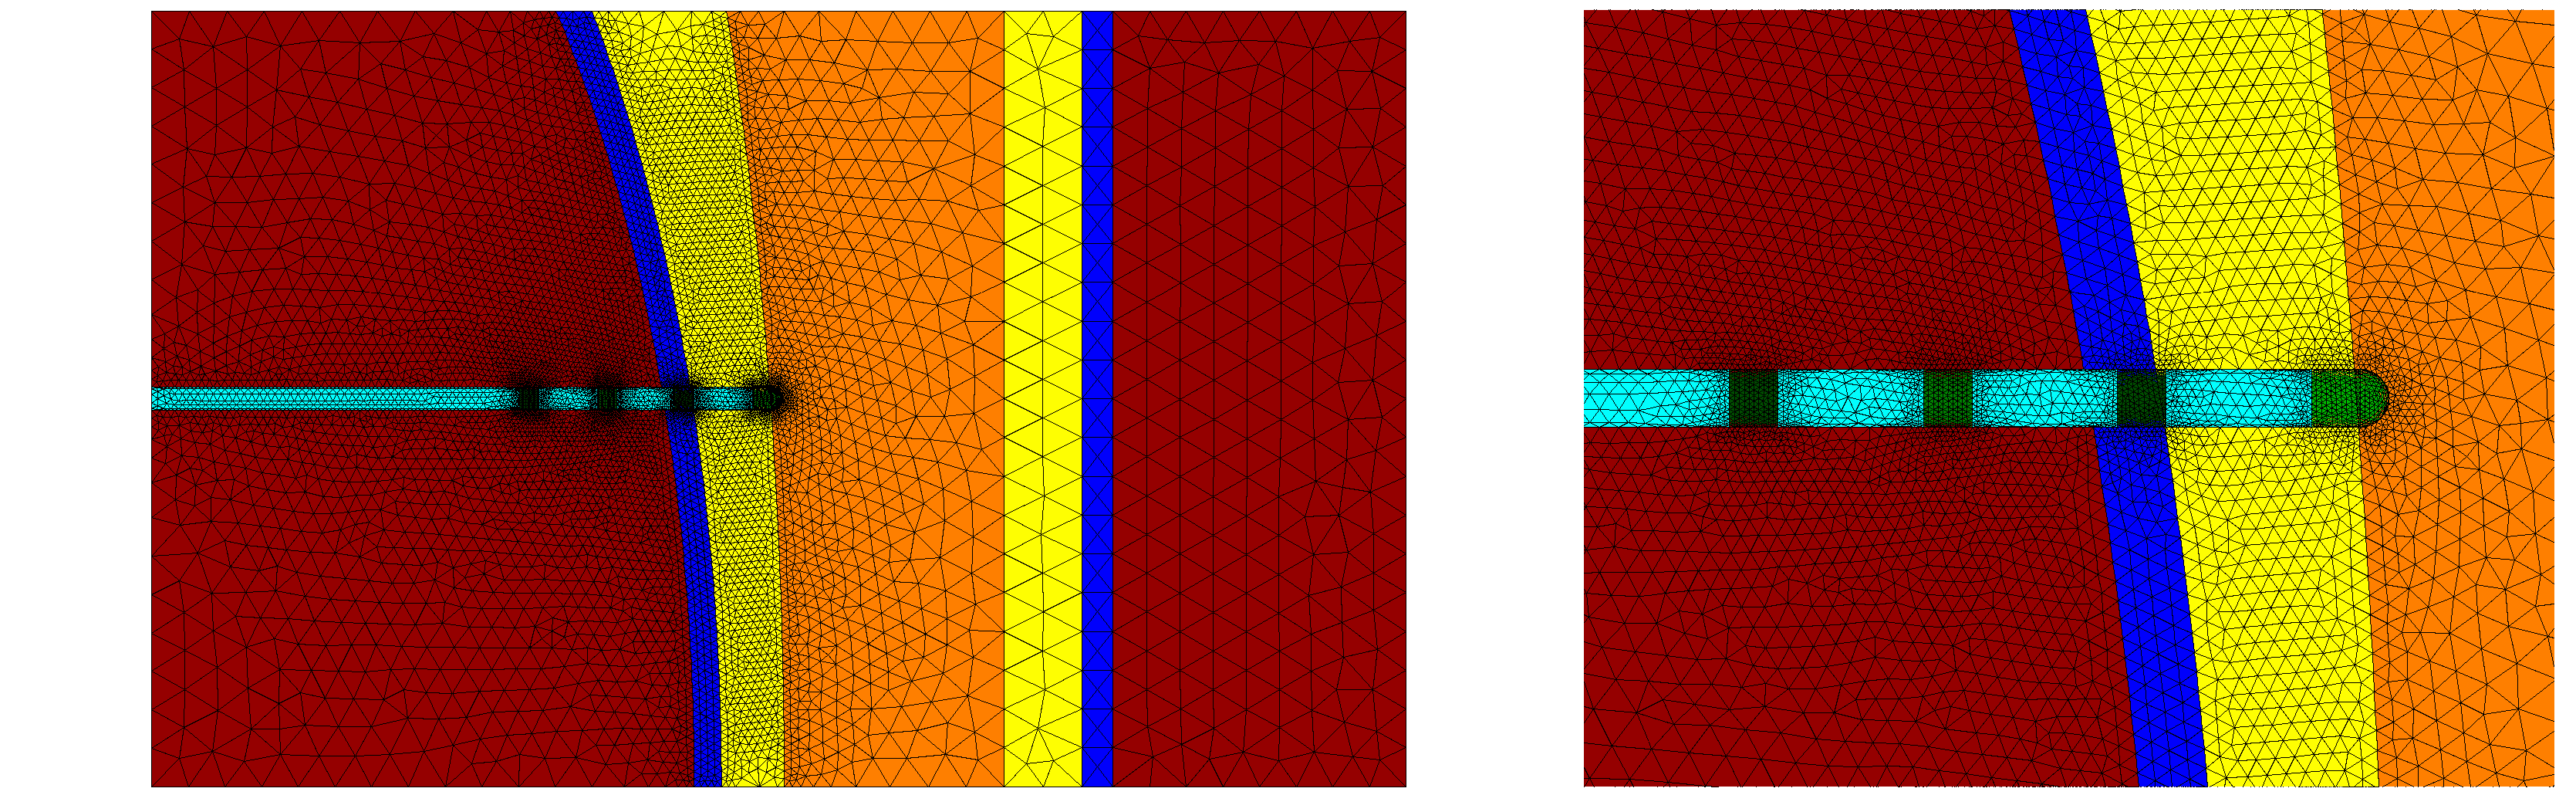
\includegraphics[width=\columnwidth]{chapter4-mesh_refinement/imgs/advanced_mesh_combined.pdf}
    \caption[Advanced mesh example of an internal probe]{\label{fig:adv_mesh} Example FEMs of a probe entering a bone from the surrounding 
    tissue. Refinement is specified around the electrodes and tissue interfaces near the probe.}
\end{figure}

Despite the increased ability to control refinement, the results still show that there are
discrepancies between the specified parameters and the resulting meshes. The data in 
\fref{tab:mesh-table} show that the maximum edge lengths specified for each mesh 
were different from the actual maximum edge lengths. As the node density was increased
near the electrodes, in Netgen the balance point did not always shift towards the electrode
as the maximum node density was not always higher despite specifying a smaller mesh size.
In Gmsh the mesh density was closer to the specified values, typically resulting in more
nodes in the refined meshes. 

Across both analyses errors away from the refined areas may be higher,
but the ability to refine meshes selectively near regions where high sensitivity 
is required may allow for reduced measurement error while still allowing for quicker 
meshing times.
As more electrodes are added and the model complexity is increased, we expect that 
refinement around the electrodes will continue to reduce total sensitivity error. However 
the node balance analysis will not be possible for irregularly shaped models.
The node balance analysis provides a straightforward method to determine the 
ideal placement for a given number of nodes to reduce model errors.

% Based on these results, we produced an additional model combining the electrode
% refinement of R8 and the maximum element size of C5 (18947 nodes and 98595
% elements). Its sensitivity
% error near the electrode was better than C2, while deeper in the medium it was
% on par with C5.  It produced measurement error of only 0.11~mV.

%\section{Conclusion}
%
%In summary, as expected, refinement of  meshes near electrodes 
%does improve model accuracy in terms of sensitivity.
%We recommend that, for each EIT imaging case, required model accuracy be
%determined from an analysis of the system, 
%and to minimize the sensitivity error in the forward solution 
%the balance of the nodes should be approximately 
%85\% towards the radius of the
%model when the dissipation of mesh refinement is constant. 

\section{Summary}
In this chapter we examine the requirement for mesh refinement around 
electrodes in Electrical Impedance Tomography (EIT). 
While it has been recommended that  models be refined around the electrodes, where current
density and sensitivity are highest,  the level of refinement required is poorly understood. 
Using a set number of nodes, we investigate the optimal distribution 
between the electrodes and 
the volume of a model. 
A balance point is used to measure the difference in distribution between the electrode and the centre of
the model.
To calculate this, all nodes contained between the surface of a selected electrode and the centre of the model 
were identified and the mean position of nodes along the container axis was computed. 
%A balance point was defined as the mean distance of all nodes along the axis 
%of a container encompassing all points between the centre of the model and the surface of a selected electrode.
We compare refinement strategies across commonly used meshing software in EIT and compare the 
model sensitivity error to an ultra-fine reference mesh. 
In a tank model, for a fixed number of nodes, error in the sensitivity calculation is minimized 
when the balance point of the nodes is n  85\% of the tank radius and the node density dissipates evenly 
from the electrode surface to the centre of the model. Using this method sensitivity error was decreased 
in all regions with high sensitivity. This node distribution technique  enables the generation  of accurate 
meshes with fewer nodes that can reduce measurement error and computing time. 
%\end{abstract}